%!TEX root = ..\Master.tex

\section{Data Gathering}
The data used in this project was gathered by recording three different persons reading the same article from the website "www.tv2.dk".
The data is comprised of 3 voice recordings with an average length of 36 seconds sampled with 44100 samples per second.
We trimmed the end of the 2 longest recordings to get the same amount of data for each class.

We only did one recording per person using the same microphone in the same room.
To get a more robust classifier, we could use more than one type of microphone and more than one room to get different background noises.
This data could also be made artificially by adding noise using a tool like MATLAB.

The voices was recorded on a single computer using the software Audacity\footnote{http://sourceforge.net/projects/audacity/} and the Lame mp3 codex\footnote{http://lame.sourceforge.net/}.
The data is then imported into matlab using the function \texttt{[data, Fs] = audioread(pathToFile)} and normalised by removing the mean of the data, and whitening the data.
The whitening is used in order to compensate for the difference in between sample volume variation. The whitening also compensates for the difference between voice clips.
The files are in stereo and both channels are used by appending one channel to the other so to have one long array of data.

\section{Feature Extraction}
Features for speaker recognition can be extracted in multiple ways. In this project two methods was used: fast Fourier transform and Mel Frequency Cepstral Coefficient method.

Fast Fourier transform (FFT) yields a frequency spectrum that is unique to each person. The frequency spectrum is divided into a series of bands with a fixed window in frequency and the resulting bands are used as features. 

The Mel Frequency Cepstral Coefficient method is commonly used to extract features in speech and speaker recognition. The methods provides features that are useful for classifying linguistic content. The basis is that the speech from humans is uniquely filtered by the shape of the vocal tract, tongue, teeth etc\footnote{http://practicalcryptography.com/miscellaneous/machine-learning/guide-mel-frequency-cepstral-coefficients-mfccs/ - retrieved 4 june 2015}. 

MFCCs are found using a series of steps as can be seen in figure \ref{fig:MFCCsteps}.
\begin{figure}[H]
\centering
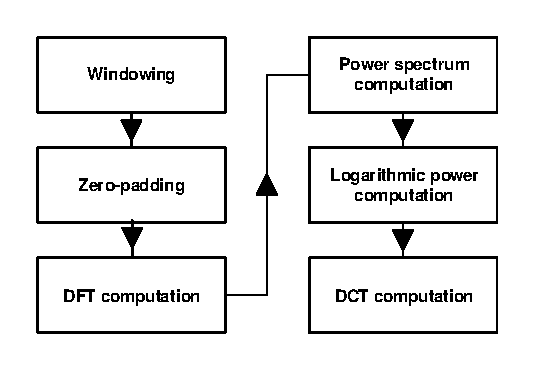
\includegraphics[scale=1]{billeder/MFCCsteps}
\caption{MFCC steps}
\label{fig:MFCCsteps}
\end{figure}
The figure has been derived from the article \cite{Sahidullah2012}. The steps can be described as follows:
\begin{enumerate}
\item Windowing: The speech signal is windows with either a Hamming or Hanning window.
\item Zero-padding: A number of zeros are padded to he windowed speech signal in order to enable FFT.
\item DFT: The windowed speech signal is discrete fourier transformed using a FFT algorithm.
\item Power spectrum: The resulting spectrum is mapped onto the mel scale but utilising a triangular filter bank.
\item Logarithmic power: The power spectrum is converted to logarithmic scale with respect to the mel frequencies.
\item DCT: The logarithmic mel powers are discrete cosine transformed. The MFCCs is the amplitudes of the output spectrum.
\end{enumerate}

In MATLAB this is done using the toolbox, voicebox\footnote{http://www.ee.ic.ac.uk/hp/staff/dmb/voicebox/voicebox.html - retrieved 6 june 2015}. The function for getting the MFCCs is called \texttt{melcepst} and a thorough explaination can be found on the voicebox website\footnote{http://www.ee.ic.ac.uk/hp/staff/dmb/voicebox/doc/voicebox/melcepst.html}. 

In short the function is invoked like this:
\begin{verbatim}
mel = melcepst(data(:,i), Fs(i), 'M0d', nc, p, n, inc);
\end{verbatim}
With \textbf{data} being the signal we want to extract the MFCCs from. 
\textbf{Fs} is the sampling frequency of the signal. 
\textbf{'M0d'} is the mode string and the three characters correspond to Hamming window, include 0'th order cepstral coefficient and include delta coefficients.
\textbf{nc} is the number of cepstral coefficients excluding 0'th coefficient.
\textbf{p} is the number of filters in the filterbank.
\textbf{n} is the length of the frame in the samples.
and lastly \textbf{inc} is the frame increment value.
\fxnote{Possible formatting of this block of text}

In this project the window size is chosen to be 200 milliseconds. The default value for speaker recognition is 150 milliseconds while speech recognition is typically lower than that. The number of cepstral coefficients was chosen to be 30.

The mel output from the function is used for features. The resulting matrix is $M \times N$ with M being number of samples of each MFCC and N being number of MFCCs. For the data used in this project this corresponds to a $2175 \times 62$.

The samples map to three classes. Class 1 will be known as Nicolai. Class 2 will be known as Reimer and lastly Class 3 will be known as Rune.


%------------------------------------------------